\documentclass{article}

\usepackage[a4paper, total={6in, 9in}]{geometry}
\usepackage{tikz}
\usetikzlibrary{shapes.geometric, arrows}
\usepackage{float}

% Generator setup

\tikzstyle{endNodes} = [rectangle, minimum width=2cm, minimum height=1cm, text centered, text
width=2cm, draw=black]

\tikzstyle{freqConverter} = [diamond, minimum width=2cm, minimum height=1cm, text centered, text
width=2cm, draw=black]

\tikzstyle{generators} = [circle, minimum width=2cm, minimum height=1cm, text centered, text
width=2cm, draw=black]

\tikzstyle{arrow} = [thick,-,>=stealth]

\title{Guest Lecture Review Craig Brown\\Ross Island Wind Farm}
\author{Jos Craw\\35046080}

\begin{document}

\maketitle{}

This lecture was presented by Craig Brown an engineer at Meridian over the course of his lecture
he discussed the engineering and management challenges associated with the design and construction
of the Ross Island Wind Farm system. Craig first discussed the conditions on Ross Island stating
that it is the highest, windiest, and coldest continent on earth. In Antarctica the frost layer is
up to 3km thick. The wind farm was designed to supplement the existing generator system and to
provide a grid between two research bases the New Zealand base, Scott Base and the American base,
McMurdo Station. The former base using 150kW and the latter using 1.6MW, the wind system was to be
used to supplement the existing diesel generator system. The proof of concept for this system was
Crater Hill, a system of three turbines with a combined output of approximately 1MW. This
installation over the last year resulted in a 1243 Tonne reduction of $CO_{2}$ output.

\begin{figure}[H]
    \centering
    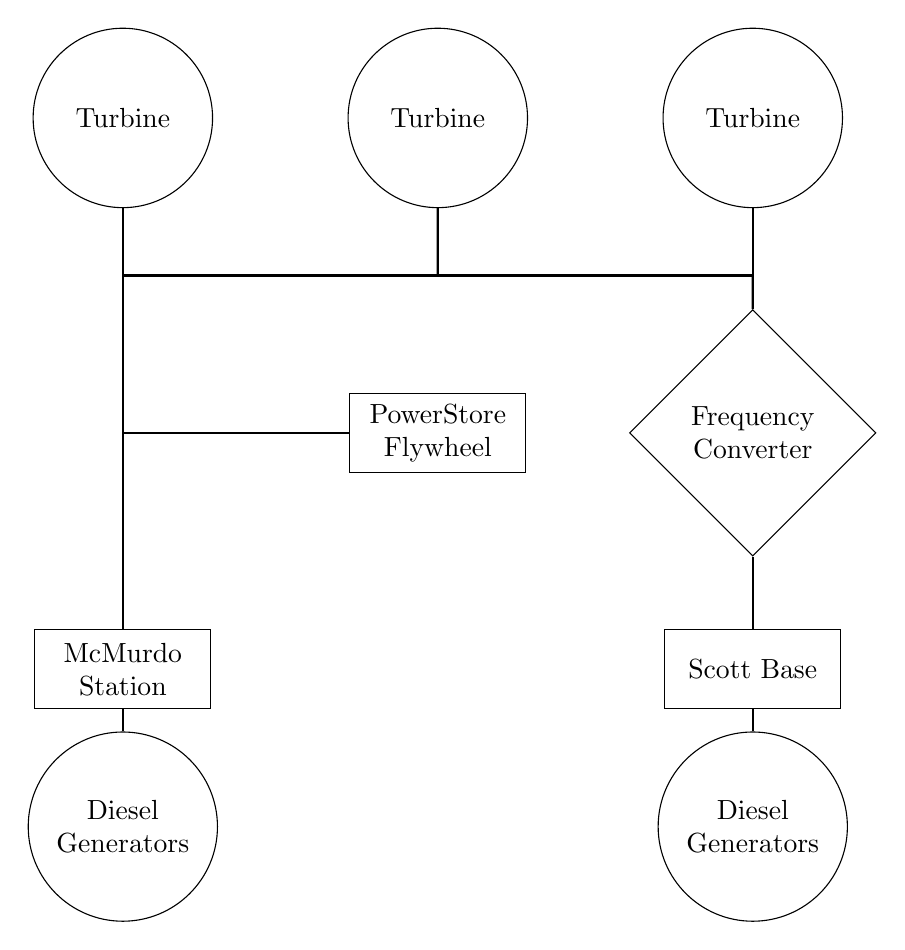
\begin{tikzpicture} [node distance=2cm]
        
        \node (turbine1) [generators] {Turbine};
        \node (turbine2) [generators, right of=turbine1, xshift=2cm] {Turbine};
        \node (turbine3) [generators, right of=turbine2, xshift=2cm] {Turbine};

        \node (flywheel) [endNodes, below of=turbine2, yshift=-2cm] {PowerStore Flywheel};
        \node (freqconvert) [freqConverter, below of=turbine3, yshift=-2cm] {Frequency Converter};

        \node (McMurdo) [endNodes, below of=flywheel, xshift=-4cm, yshift=-1cm] {McMurdo Station};
        \node (Scott) [endNodes, below of=freqconvert, yshift=-1cm] {Scott Base};

        \node (ScottGen) [generators, below of=Scott] {Diesel Generators};
        \node (McMurdoGen) [generators, below of=McMurdo] {Diesel Generators};

        \draw[arrow] (McMurdoGen) -- (McMurdo);
        \draw[arrow] (McMurdo) -- (turbine1);
        \draw[arrow] (McMurdo) |- (flywheel);

        \draw[arrow] (McMurdo) |- (4, -2);
        \draw[arrow] (4, -2) -- (turbine2);
        \draw[arrow] (4, -2) -| (turbine3);

        \draw[arrow] (freqconvert) -- (8, -2);
        \draw[arrow] (Scott) -- (freqconvert);
        \draw[arrow] (ScottGen) -- (Scott); 

    \end{tikzpicture}
    \caption{Crater Hill System}
\end{figure}

Craig then told us about some design issues that were occurred during the project. The first was
the permafrost the was just 45cm under the surface. This layer had to be remove with dynamite and
quickly excavated before it could refreeze. The next major issue was the transport of the
materials required for construction, these could only be brought in on one ship once per year,
meaning that if cargo wasn't on the ship it would not be able to be shipped until the next year.
This could potentially delay the project by a full year. Another issue with transportation was the
conditions for transport, the sea could be extremely rough, this happen with this project where
the shipping container containing the crane was damaged during transport. Luckily due to the part
being slightly smaller than the crate there was not damage to the part. Another major design issue
was building the system to meet standards, this proved difficult particularly for grounding as the
resistance was much higher than the standards at 104 Ohms. These standards were in place to
protect from lightning strikes, this however is not an issue in the Antarctic as it is much too
dry. Therefore the project had to explain that the design met the outcomes of the standards, just
not the standards themselves. Another difficulty encountered was an IGBT failure which destroyed
control boards that are no longer manufactured. This meant that the boards had to be rebuilt for
this project. Another issue with the design was the distributed control system as the American
teams did not like having a system with no master controller. This issue was fixed by ensure the
system had modes to deal with certain systems being unresponsive.

Craig then covered his specific role in the project, he is a Project Electrical Engineer. In this
position Craig handles design approval, procurement and medium voltage equipment specification and
procurement. Craig is also a Contract supervisor where he handles quality assurance, ensuring
specifications are meet, as well as ensuring that the design is installed correctly.

Craig told us about the design is now operating and had produced 29.1GWh from the end of June
2019, with 77\% delivered to McMurdo Station. Scott Base now has completely automated
power generation. The turbines 2.478GWh which was 78\% of the projected output this decrease in
output was due to a power store IGBT failure as well as some turbine faults and turbine
inspections.

Finally, the design principals were discussed. These are as follows:
\begin{itemize}
    
    \item{Cost}
        \begin{enumerate}
            \item{Find cheaper method}
            \item{Projects always have budgets}
        \end{enumerate}

    \item{Solutions}
        \begin{enumerate}
            \item{Find solutions}
            \item{For this project, the team was unable to give up due to the profile of the
                project the company would look bad}
        \end{enumerate}

    \item{Fit for Purpose}
        \begin{enumerate}
            \item{Ensure all equipment is fit for its specific purpose}
            \item{For this project the specific conditions must be considered}
        \end{enumerate}

    \item{Future}
        \begin{enumerate}
            \item{Plans for future expansion must be considered}
            \item{For this project production increase the amount of carbon release will greatly
                decrease}
        \end{enumerate}

    \item{Learn From past mistakes}

    \item{Practicality}
        \begin{enumerate}
            \item{Simplicity is key}
            \item{Make sure the design is easy to install}
        \end{enumerate}

    \item{Maintainability}
        \begin{enumerate}
            \item{Reduce maintenance requirements}
            \item{For this project maintenance with simple tools was a requirement due to the
                remoteness of the location}
        \end{enumerate}

    \item{Consider constraints}
        \begin{enumerate}
            \item{This was a multinational project so language and units as well a differing phase
                colours were an issue}
            \item{The environmental conditions of the region were a major constraint}
            \item{The time frames for this project were tight as shipping components could only
                occur once per year}
        \end{enumerate}

\end{itemize}

These design principals were the major take homes for this lecture as these are all things that
should be considered for our designs in the future as while our projects may be less extreme in
nature these principals will all have to be considered.
\end{document}

